% !TeX root = ../thuthesis-example.tex

\chapter{信息聚类理论与算法}
数据聚类方法与社群发现方法有着天然的联系。

\section{社群发现场景下的多变量互信息理论}
在这一节中,我们首先把\ref{sec:local_geometry}节介绍
的弱独立的概念推广到多个随机变量弱独立,
并在多个随机变量弱独立的条件下,对
\ref{sec:info_clustering}节介绍的多变量互信息
进行化简。
\begin{definition}\label{def:general}
  称$Z_1, \dots, Z_n (n\geq 2)$
  是$\epsilon$-弱独立的,如果存在一个随机变量 $U$
  使得
  $(Z_1, \dots, Z_n)|U$的PMF 在 $(Z_1, \dots, Z_n)$的
  $\sqrt[n]{\epsilon}$邻域内并且
  $Z_1, \dots Z_n$关于
  $U$的条件分布是独立的。
  \end{definition}
\begin{example}\label{ex:xy_weak_ext}
    考虑例 \ref{ex:Pweak_1}给出的分布,给定$X,Y$
    的分布为$P(x,y)=\frac{1}{4}(1+\epsilon(-1)^{x+y})$。
    我们构造一分布$U$如表所示:
    \begin{table}
      \begin{tabular}{|c|c|c|c|c|}
        \hline
        $P(U=i|X=j, Y=k)$ & $j=0,k=0$ &
        $j=0,k=1$ & $j=1,k=0$  & $j=1,k=1$ \\
        \hline
        $i=0$ & $\frac{(1-\sqrt{\epsilon})^2}{2(1+\epsilon)}$
        & $\frac{1}{2}$ & $\frac{1}{2}$ 
        &  $\frac{(1+\sqrt{\epsilon})^2}{2(1+\epsilon)}$\\
        \hline
        $i=1$ & $\frac{(1+\sqrt{\epsilon})^2}{2(1+\epsilon)}$
        & $\frac{1}{2}$ & $\frac{1}{2}$
        & $\frac{(1-\sqrt{\epsilon})^2}{2(1+\epsilon)}$
        \\
        \hline
      \end{tabular}
    \end{table}

    不难验证$P(X=j, Y=k | U=i)=P(X=j | U=i)
      P(Y=k| U=i)$。此外, $(X, Y)|U=0$
      的PMF 可以写成向量的形式
      $\frac{1}{4}[(1-\sqrt{\epsilon})^2,
      1-\epsilon,
      1-\epsilon,
      (1+\sqrt{\epsilon})^2]$,它在
      $(X,Y)$的PMF 向量
      $\frac{1}{4}[1+\epsilon, 1-\epsilon, 1-\epsilon, 1+\epsilon]$
      的 $\sqrt{\epsilon}$-邻域内。因此
      $X,Y$是$\epsilon$-弱独立的。
\end{example}
例\ref{ex:xy_weak_ext}展示了定义\ref{def:general}和
定义\ref{def:weak_indepedent}在两变量情形的一个共用的例子。
事实上,我们可以证明定义\ref{def:general}是
定义\ref{def:weak_indepedent}的拓展。
\begin{theorem}\label{thm:weak_independence_equivalent}
  如果 对于任何 $x \in \mathcal{X}$,
$Y$关于$X$的条件 PMF 
$P_{Y|X}(\cdot |x)$在$Y$的$\epsilon$邻域内,那么存在
一个随机变量 $U$
  使得
  $(X, Y)|U$的PMF 在 $(X, Y)$的
  $\sqrt{\epsilon}$邻域内并且
  $X, \dots Y$关于
  $U$的条件分布是独立的。
\end{theorem}
\begin{proof}
  由$\epsilon$邻域的定义式\ref{def:eps_neighborhood},
  $P_{Y|X=x}(y) = P_Y(y) + \sqrt{P_Y(y)}\phi_{Y|X=x}(y)
  \epsilon$。定义$\phi_{XY}(x,y)=\sqrt{P_X(x)}\phi_{Y|X=x}(y)$
  则有
  $P_{XY}(x,y) = P_X(x)P_Y(y) + \sqrt{P_X(x)}\sqrt{P_Y(y)}\phi_{XY}(x,y)
  \epsilon$。
  假设$x\in \mathcal{X}$ 且 $y\in \mathcal{Y}$,
  $\mathcal{X}, \mathcal{Y}$ 均为有限的字母集。
  $\phi_{XY}$ 是 $|\mathcal{X}| \times |\mathcal{Y}|$
  的矩阵,其秩为 $r$。可以通过$SVG$分解为
  $\frac{1}{r}\sum_{i=1}^r \phi_i \psi^T_i$,其中$\phi, \psi$
  分别为长度为$|\mathcal{X}|, |\mathcal{Y}|$的
  列向量。构造 $U$ 是$\{1, 2, \dots, 2r\}$ 上面的均匀分布。
  $Z_1, Z_2$ 做如下构造:
  \begin{align*}
    P(Z_1=x|U=i) &= P_X(x) + (-1)^i\sqrt{P_X(x)}\phi_{\lceil i/2 \rceil}(x) \sqrt{\epsilon}, x \in \mathcal{X} \\
    P(Z_2=y|U=i) &= P_Y(y) + (-1)^i\sqrt{P_Y(y)}\psi_{\lceil i/2 \rceil}(y) \sqrt{\epsilon}, y \in \mathcal{Y}\\
  \end{align*}
  $Z_1 | U$ 与$Z_2 | U$ 独立,因此,
  $Z_1, Z_2$ 的联合分布为:
  \begin{align*}
  P(Z_1=x, Z_2=y)& =\sum_{i=1}^{2r}P(U=i)P(Z_1=x|U=i)P(Z_2=y|U=i)\\
  &=P_X(x)P_Y(y) + \sqrt{P_X(x)}\sqrt{P_Y(y)}\frac{\epsilon}{r}
  \sum_{i=1}^{r}\phi_i(x)
  \psi(y) =P(X=x,Y=y)
  \end{align*}
  因此,$Z_1, Z_2$与$X,Y$具有相同的分布。
  不难验证$(Z_1, Z_2)|U$在$(Z_1, Z_2)$的$\sqrt{\epsilon}$邻域内,
  故结论得证。
  \end{proof}
  定理\ref{thm:weak_independence_equivalent}的证明提供了一种生成
  满足弱独立条件的随机变量的方法。即给定均匀分布
  $U$ 在 $n! \times r$个点上取值,
  并且$Z_i|U$在分布$Z_i$的
  $\sqrt[n]{\epsilon}$ 邻域内:
  \begin{equation}
    P(Z_j=z|U=i) = P_{Z_j}(z) + 
    (-1)^{i \,\mathrm{mod}\, n!}\sqrt{P_{Z_j(z)}}
    \phi_{\lceil\, i/n!\, \rceil}(z) \sqrt[n]{\epsilon}, z \in \mathcal{Z_j}
  \end{equation}
  假设$Z_1|U, \dots, Z_n|U$ 独立,可得到
  $(Z_1, \dots, Z_n)|U$的分布。
  不然验证通过这种方法构造出来的分布$Z_1, \dots, Z_n$是弱独立的。

与\ref{sec:info_clustering}节介绍的 PIN 模型类似,
在多个随机变量弱独立的条件下,KL散度的计算可以
与图结构进行对应。即有如下定理:
\begin{theorem}\label{thm:DPX}
若 $Z_1, \dots, Z_n$ $\epsilon$-弱独立, 则有
\begin{equation}\label{eq:PXV}
D(P_{Z_V} || \prod_{C\in \P} P_{Z_{C}}) = {1 \over 2}
\sum_{\substack{(i,j) \not\in C\\ C\in \P}} \norm{B_{ij}}_F^2 + o(\epsilon^2)
\end{equation}
其中 $B_{ij}$ 是 随机变量  $Z_i$ 和 $Z_j$
之间的$B$ 矩阵(参见式\ref{eq:Ixy})而 $\P$是$V$的一个分割(
参见式\ref{eq:IPZV})。 
\end{theorem}
若$ n = 2$,定理\ref{thm:DPX} 即是用 $B$ 矩阵估计互信息,
与 式 \eqref{eq:Ixy} 相同。
因此,定理\ref{thm:DPX}可看成式 \eqref{eq:Ixy} 
的拓展。

定理 \ref{thm:DPX} 是关于弱独立的随机变量的。
现在我们把它拓展到针对数据样本。
给定一 $K$ 个聚类簇的数据集,一共有 $n$ 个样本。
每个 聚类簇被看成一个随机变量。
假设第 $i$ 个 聚类簇 $Z_i$ 字母集 为 $\abs{\mathcal{Z}_i}$,
全局约束是 $\sum_{i=1}^K \abs{\mathcal{Z}_i} = n$。
假设$Z_1, \dots, Z_K$弱独立,
由弱独立的定义式 \ref{def:general}, $Z_i$ 和 $Z_j$ $\epsilon$-弱独立 ($i\neq j$),
于是我们有
\begin{equation}\label{eq:phi_w}
P_{Z_i Z_j}(z_i, z_j) = P_{Z_i}(z_i)P_{Z_j}(z_j) + \epsilon \sqrt{P_{Z_i}(z_i)P_{Z_j}(z_j)} \phi_{Z_i Z_j}(z_i, z_j) + o(\epsilon)
\end{equation}
因此,由 \eqref{eq:Ixy}式,
 $\norm{B_{ij}}_F^2 = \epsilon^2 \sum_{z_r \in \mathcal{Z}_i, z_s \in \mathcal{Z}_j} \phi^2_{Z_i Z_j}(z_r, z_s)$ 
 并且 式 \eqref{eq:PXV} 可以展开成
\begin{equation}\label{eq:PXV_Data}
D(P_{Z_V} || \prod_{C\in \P} P_{Z_{C}}) =
{\epsilon^2\over 2}\sum_{\substack{(i,j) \not\in C\\ C\in \P}}
\sum_{z_r \in \mathcal{Z}_i, z_s \in \mathcal{Z}_j}  \phi^2_{Z_i Z_j}(z_r, z_s) + o(\epsilon^2)
\end{equation}
我们可以把
$\phi^2_{Z_i Z_j}(z_r, z_s)$ 这一项
当成一个有$n$个节点的图的
边的权值。
图的每一个节点对应一个数据点。
为简化符号, 令 $w_{rs} = \phi^2_{Z_{d(z_r)}Z_{d(z_s)}}(z_r, z_s)$
\footnote{当 $d(z_r) = d(z_s)$ 时,
我们仍可以形式化的定义 $w_{rs}$ 为远大于$\max\{\phi^2_{Z_i Z_j}(z_r, z_s), i\neq j\}$
的值。},
其中,$d(z_r)$ 把节点映射到它所属的随机变量的序号, 定义域 为 $1\leq r,s \leq \abs{V}$。
我们也可以展开 每个 $Z_i$ 到它的节点集 并且将分割 $\P$
看成是对节点集的分割。
假设我们考虑的图 $G(V, E)$ 是有向的
\footnote{有向图的假设可以减少计算量而不失一般性},
类似 式 \ref{eq:IP} 我们定义图的入割函数 (in-cut function) $f(C)$ for $C\subseteq V$ as $f(C) = \sum_{i\not\in C, j\in C, (i,j) \in E} w_{ij}$,
它是所有进入$C$的有向边的权值之和。
基于上面定义的符号,表示KL散度的式 \eqref{eq:PXV_Data} 可以写成聚类簇之间边的权值之和
的形式:
\begin{equation}\label{eq:PXV_Data_Simplified}
D(P_{Z_V} || \prod_{C\in \P} P_{Z_{C}}) = \epsilon^2 \sum_{C \in \P} f(C)+ o(\epsilon^2)
\end{equation}
从而我们获得了在多变量弱独立条件下数据聚类的表达式。
由于$\epsilon$是给定的无穷小量,我们更关心$\epsilon^2$
的系数,该系数即与式\eqref{eq:IP}中的$f[\P]$一样,
也在我们求解等价的优化问题式\eqref{eq:hlambda}中出现过。
\section{与数据聚类问题的联系}
社群发现是输入一张图获得节点所属的类别,而
数据聚类的任务与社群发现相同,但其输入是一个数据矩阵,
其中行数是数据的个数而
每一行的向量代表该数据的特征。二者可以通过
输入数据的格式转换来实现算法互通。一般而言,
从数据矩阵到图的变换是可以通过选取一
相似度度量$d(\cdot,\cdot)$作用到数据上
获得图中边的权值,即$w_{ij}=d(x_i, x_j)$。
在这一节中,
我们研究的重点是如何用
\eqref{eq:hlambda} 实现数据聚类的任务。
在永野清仁的文章中\cite{mac},已经有用RBF核作为相似度度量的
尝试,但局限于该相似度度量在小规模真实世界数据集上表
现不佳,此外相似度度量本身具有一些超参数,也会影响聚类
效果。我们通过使用交叉验证、网格搜索,及对
不同相似度度量的枚举,试图寻找特定问题下具有
较好表现的相似度度量及其超参数。

我们使用5种数据集对基于图分割的数据聚类方法
进行测试,各数据集的基本情况如表\ref{tab:clustering_dataset}
所示。
\begin{table}[!ht]
  \centering
  \begin{tabular}{|c|c|c|c|}
    \toprule
    名称 & 样本数量 & 类别数量 & 特征维度 \\
    \midrule
    Gaussian & 100 & 4 & 2 \\
    Circle & 300 & 3 & 2 \\
    Iris & 150 & 3 & 4 \\
    Glass & 214 & 6 & 9 \\
    Libras & 360 & 15 & 90 \\
    \bottomrule
  \end{tabular}
  \caption{数据聚类测试数据}\label{tab:clustering_dataset}
\end{table}
其中,Gaussian 和 Circle 是人工生成的数据集。
Iris, Glass 和 Libras 是来自 UCI 机器学习标准数据集
\cite{Dua:2019}。

首先我们展示在两个人工生成的数据集上的聚类效果,
Gaussian 数据集的相似度度量取 式\ref{eq:rbf_kernel} 所示的 RBF 核,
$\gamma=0.6$。
\begin{equation}\label{eq:rbf_kernel}
  w_{ij}=\exp(-\gamma ||x_i-x_j||^2)
\end{equation}
Circle 数据集的相似度度量通过 k近邻 进行计算,即仅与自己距离最近的$k$
个数据点有边相连\footnote{所有边权值均为1},取$k=7$。
聚类效果如图 \ref{fig:artificial_dataset_effect} 所示。

\begin{figure}[!ht]
  \begin{subfigure}[b]{\linewidth}
  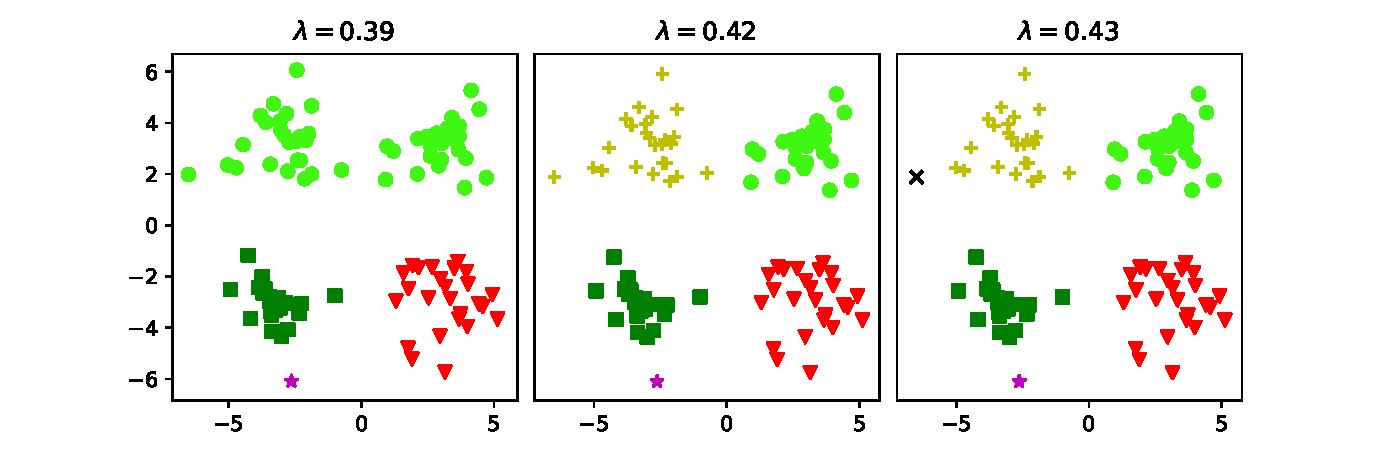
\includegraphics[width=\textwidth]{4part.pdf}
  \caption{有4个类别的 Gaussian 数据集}
  \label{fig:4p}
\end{subfigure}
\begin{subfigure}[b]{\linewidth}
  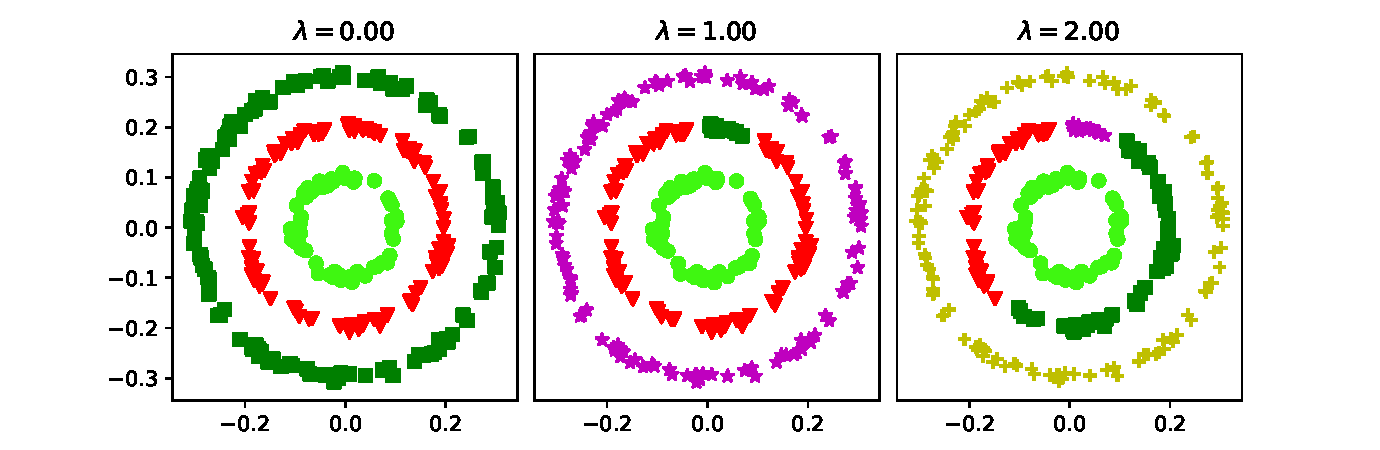
\includegraphics[width=\textwidth]{3circle.pdf}
  \caption{有3个类别的 Circle 数据集}
  \label{fig:3c}
\end{subfigure}
\caption{人工生成的数据集聚类效果}
\label{fig:artificial_dataset_effect}
\end{figure}

从图中可以看到,通过选取适当的阈值 $\lambda$,
可获得与数据的真实类别十分接近的聚类结果,对应于图
\ref{fig:4p} 中的 $\lambda=0.42$
和图\ref{fig:3c} 中的 $\lambda=0.0$。

\section{基于图分割的社群发现算法及其改进}
在本节中,我们首先介绍我们对PSP算法的改进,并在一定
的假设下证明其理论复杂度,最后比较求解图分割的三种不同实现下
的算法效率。

我们改进的PSP算法仍将使用
算法 \ref{alg:psp} 中提到的
\texttt{DT} 子函数。
在算法\ref{alg:psp} 中,我们观察到
每次调用 \texttt{DT} 是相互独立的,
并没有利用到聚类树的 固有性质。
如果聚类树的嵌套性质可以被考虑进来的话, 
我们可以在后面的计算中
仅在子图上进行 \texttt{DT} 的调用,
从而可以实现计算效率比PSP算法提升一个数量级。


具体来说,
假设我们第一次调用DT后得到了
$P_i = \{C_1, \dots, C_t\}$。
然后我们 分别对每个
$C_i(i=1,\dots, t)$
计算 PSP分割。
并从子图的计算中构造 $P_j(j>i)$。
对于 $P_j(j<i)$,
我们可以把 图 $G$
缩成 图 $G^t$,其中 每个$C_i$集合中的点缩成一个单独的节点。
因此图 $G^t$共有 $t$ 个节点。
通过在$G^t$ 上调用 DT 函数我们可以得到  $P_j(j<i)$。
我们把我们的改进方法称为 HPSP,其中 H 表示 “层次的”
英文首字母\footnote{hierarchical},
其描述在算法\ref{alg:psp_i_simplified}中给出。

\begin{algorithm}
	\caption{改进的求解主分割序列的算法}\label{alg:psp_i_simplified}
	\begin{algorithmic}[1]
		\REQUIRE 有向图 $G(V, E)$; 边的权值函数 $w(e)$,其中 $e\in E$
		\ENSURE 聚类树 $\mathcal{T}(K, E)$ 其中 $K \subseteq 2^{V}$ 表示节点集
    而 $E$ 表示边的集合。
		\STATE 初始化 树 $\mathcal{T}$:
     $V$ 是根节点,
     $\{j\}(j \in V)$ 是诸叶节点,
     无其他节点。
		\STATE \texttt{Split}($G, V$)
		\FUNCTION{\texttt{Split}($\widetilde{G}, \widetilde{V}$)}
		\STATE $w$ 是 $\widetilde{G}$ 所有边的权值之和。
		\STATE $\gamma' = \frac{w}{\abs{V(\widetilde{G})}-1}$
    其中 $V(\widetilde{G})$ 是 图$\widetilde{G}$
    的节点集。
    \label{alg:gamma_apostrophe}
		\STATE $(\tilde{h}, P') = \texttt{DT}(\widetilde{G}, \gamma')$ 其中
    $\P'$ 是在 式 \eqref{eq:hlambda} 中达到
    最小值 $h(\gamma')$的分割
    并且 $\tilde{h}$ 是对应的最小值。 \label{line:DT}
		\IF{$\tilde{h} = - \gamma'$}
		\STATE 在聚类树
    $\mathcal{T}$ 中把权值 $\gamma'$ 标记在从 $\widetilde{V}$ 出发
    到其所有子节点的边上。
		\ELSE
		\FOR{$S$ in $P'$ and $\abs{S}>1$}
		\STATE 在聚类树
    $\mathcal{T}$ 中构造新的节点$S$,并修改 $\widetilde{V}$的子节点的父亲节点 为$S$,
    而$S$的父节点为$\widetilde{V}$。
		\STATE \texttt{Split}($\widetilde{G}[S], S$)
    其中 $\widetilde{G}[S]$ 是 $\widetilde{G}$ 限制在 $S$
    上的子图。\label{line:SplitDown}
		\STATE 在 $\widetilde{G}$ 中将 $S$ 缩成一个节点。 % graph \widetilde{G} is modified
		\ENDFOR 
		\STATE \texttt{Split}($\widetilde{G}, \widetilde{V}$)		\label{line:SplitUp}
		\ENDIF
		\ENDFUNCTION
	\end{algorithmic}
\end{algorithm}

\begin{figure}[!ht]
	\centering
	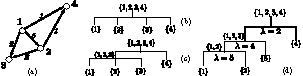
\includegraphics[width=10cm]{alg_illustration.pdf}
	\caption{HPSP 求解图(a)的主分割序列,聚类树经(b), (c) 演化到 (d) }\label{fig:alg_eg}
\end{figure}

\begin{example}
	We use a simple example to explain Algorithm \ref{alg:psp_i_simplified}. Consider a graph $G(V, E)$ with $V=\{1,2,3,4\}, E=\{(1,2),(1,3),(2,3),(1,4),(2,4)\}$. The weight values are $w_{13}=2, w_{12}=5, w_{23}=2, w_{14}=1, w_{24}=1$. The graph is illustrated
	in Fig. \ref{fig:alg_eg} (a). Initially, the hierarchical tree is shown in Fig. \ref{fig:alg_eg} (b). Computing $\gamma' = \frac{11}{4-1}, \tilde{h} = -\frac{16}{3} < -\gamma' $ and $\P' = \{\{1,2,3\},\{4\}\}$ from line \ref {alg:DT} in Algorithm \ref{alg:psp_i_simplified} we get the hierarchical tree shown in Fig. \ref{fig:alg_eg} (c).
	
	Then we run PSP for the subgraph $G[\{1,2,3\}]$, $\gamma' = \frac{9}{2}, \tilde{h} = -5 < -\gamma'$ and $\P= \{\{1,2\},\{3\}\}$ we get the tree shown in Fig. \ref{fig:alg_eg} (d). Other computation gives the edge weight of $\mathcal{T}$ shown in Fig. \ref{fig:alg_eg} (d).
\end{example}	
\section{基于图分割的社群发现算法在异常值检测领域的应用}

\section{代码实现}
尽管最大流算法包比较多,但我们尚未发现
求解层次分割(式\eqref{eq:PSP_structure})的开源实现。
因此我们使用 C++ 实现了跨平台的PSP算法\ref{alg:psp}
(内嵌迪尔沃思截断算法\ref{alg:dt}),并且
我们提供了Python编程语言的接口函数,并在 \url{pypi.org}
平台上以 pspartition
的名字发布,以供后面的研究者使用。
我们的实现使用 CMake 编译,依赖于第三方库 LEMON \cite{dezsHo2011lemon}。 
LEMON 库在我们的算法包中用于构建所需的图数据结构和最大流算法。
这里顺便提及的一点是 LEMON 库里使用的
最大流算法是基于最大标签选择策略的前置推送-标签重贴算法。
根据文献\citet{ahuja1997computational}的比较,该算法
的效率比起其他解最大流问题的算法有明显的优势。

在Python的接口函数方面,我们采用了CPython
跨语言编程的方式,将由 NetworkX \cite{SciPyProceedings_11} 构建的图
转换成用边表示的图传递到C++中的类构造函数中,
计算完成后再把C++中的集合转换成Python中的列表
进行返回。用于求解例 \ref{ex:psp}
的示例 Python 代码如下。
\begin{lstlisting}[language=Python]
  from pspartition import PsPartition
  a = [[0,1,1], [0,2,5], [1,2,1]] # a graph
  p = PsPartition(3, a) # 3 nodes
  p.run()  
  cv = p.get_critical_values()
  pl = p.get_partitions()
  print(cv)
  print(pl)
  \end{lstlisting}
\section{实验结果}


中文论文的数学符号默认遵循 GB/T 3102.11—1993《物理科学和技术中使用的数学符号》
\footnote{原 GB 3102.11—1993,自 2017 年 3 月 23 日起,该标准转为推荐性标准。}。
该标准参照采纳 ISO 31-11:1992 \footnote{目前已更新为 ISO 80000-2:2019。},
但是与 \TeX{} 默认的美国数学学会(AMS)的符号习惯有所区别。
具体地来说主要有以下差异:
\begin{enumerate}
  \item 大写希腊字母默认为斜体,如
    \begin{equation*}
      \Gamma \Delta \Theta \Lambda \Xi \Pi \Sigma \Upsilon \Phi \Psi \Omega.
    \end{equation*}
    注意有限增量符号 $\increment$ 固定使用正体,模板提供了 \cs{increment} 命令。
  \item 小于等于号和大于等于号使用倾斜的字形 $\le$、$\ge$。
  \item 积分号使用正体,比如 $\int$、$\oint$。
  \item 行间公式积分号的上下限位于积分号的上下两端,比如
    \begin{equation*}
      \int_a^b f(x) \dif x.
    \end{equation*}
    行内公式为了版面的美观,统一居右侧,如 $\int_a^b f(x) \dif x$ 。
  \item
    偏微分符号 $\partial$ 使用正体。
  \item
    省略号 \cs{dots} 按照中文的习惯固定居中,比如
    \begin{equation*}
      1, 2, \dots, n \quad 1 + 2 + \dots + n.
    \end{equation*}
  \item
    实部 $\Re$ 和虚部 $\Im$ 的字体使用罗马体。
\end{enumerate}

以上数学符号样式的差异可以在模板中统一设置。
另外国标还有一些与 AMS 不同的符号使用习惯,需要用户在写作时进行处理:
\begin{enumerate}
  \item 数学常数和特殊函数名用正体,如
    \begin{equation*}
      \uppi = 3.14\dots; \quad
      \symup{i}^2 = -1; \quad
      \symup{e} = \lim_{n \to \infty} \left( 1 + \frac{1}{n} \right)^n.
    \end{equation*}
  \item 微分号使用正体,比如 $\dif y / \dif x$。
  \item 向量、矩阵和张量用粗斜体(\cs{symbf}),如 $\symbf{x}$、$\symbf{\Sigma}$、$\symbfsf{T}$。
  \item 自然对数用 $\ln x$ 不用 $\log x$。
\end{enumerate}


英文论文的数学符号使用 \TeX{} 默认的样式。
如果有必要,也可以通过设置 \verb|math-style| 选择数学符号样式。

关于量和单位推荐使用
\href{http://mirrors.ctan.org/macros/latex/contrib/siunitx/siunitx.pdf}{\pkg{siunitx}}
宏包,
可以方便地处理希腊字母以及数字与单位之间的空白,
比如:
\SI{6.4e6}{m},
\SI{9}{\micro\meter},
\si{kg.m.s^{-1}},
\SIrange{10}{20}{\degreeCelsius}。



\section{数学公式}

数学公式可以使用 \env{equation} 和 \env{equation*} 环境。
注意数学公式的引用应前后带括号,建议使用 \cs{eqref} 命令,比如式\eqref{eq:example}。
\begin{equation}
  \frac{1}{2 \uppi \symup{i}} \int_\gamma f = \sum_{k=1}^m n(\gamma; a_k) \mathscr{R}(f; a_k)
  \label{eq:example}
\end{equation}
注意公式编号的引用应含有圆括号,可以使用 \cs{eqref} 命令。

多行公式尽可能在“=”处对齐,推荐使用 \env{align} 环境。
\begin{align}
  a & = b + c + d + e \\
    & = f + g
\end{align}



\section{数学定理}

定理环境的格式可以使用 \pkg{amsthm} 或者 \pkg{ntheorem} 宏包配置。
用户在导言区载入这两者之一后,模板会自动配置 \env{thoerem}、\env{proof} 等环境。

\begin{theorem}[Lindeberg--Lévy 中心极限定理]
  设随机变量 $X_1, X_2, \dots, X_n$ 独立同分布, 且具有期望 $\mu$ 和有限的方差 $\sigma^2 \ne 0$,
  记 $\bar{X}_n = \frac{1}{n} \sum_{i+1}^n X_i$,则
  \begin{equation}
    \lim_{n \to \infty} P \left(\frac{\sqrt{n} \left( \bar{X}_n - \mu \right)}{\sigma} \le z \right) = \Phi(z),
  \end{equation}
  其中 $\Phi(z)$ 是标准正态分布的分布函数。
\end{theorem}
\begin{proof}
  Trivial.
\end{proof}

同时模板还提供了 \env{assumption}、\env{definition}、\env{proposition}、
\env{lemma}、\env{theorem}、\env{axiom}、\env{corollary}、\env{exercise}、
\env{example}、\env{remar}、\env{problem}、\env{conjecture} 这些相关的环境。
